\documentclass[12pt]{article}
\usepackage[utf8x]{inputenc}
\usepackage[T1, T2A]{fontenc}
\usepackage{fullpage}
\usepackage{multicol, multirow}
\usepackage{tabularx}
\usepackage{ulem}
\usepackage{listings}
\usepackage[english, russian]{babel}
\usepackage{tikz}
\usepackage{pgfplots}
\usepackage{indentfirst}
% \usepackage{noindentafter}
\usepackage{nonfloat}
\usepackage{ulem}
\usepackage{fancyhdr}
% \usepackage{courier}
% \usepackage{FiraMono}
\usepackage{color}
\usepackage{subcaption}
\usepackage{titlesec}


\parindent=1cm

\linespread{1}
\pgfplotsset{compat=1.16}
\newcommand{\se}[1]{\section*{\bf #1}}

\newcommand{\listsource}[2]{
	\subsection*{\textbf{#2}}
	{\footnotesize
	\lstinputlisting[language=lisp]{#1/#2}
	}
}

\lstdefinestyle{empty}{language=c++,
	basicstyle=\scriptsize,
	showspaces=false,
	showstringspaces=false,
	showtabs=false,
	tabsize=4,
	breaklines=true,
	escapechar=@,
	numbers=none,
	frame=none,
	escapeinside={\%*}{*)},
	breakatwhitespace=false % переносить строки только если есть пробел
}

\lstdefinestyle{customc}{
  belowcaptionskip=1\baselineskip,
  breaklines=true,
  frame=L,
  xleftmargin=\parindent,
  language=lisp,
  numbers=left,
  showstringspaces=false,
  basicstyle=\footnotesize\ttfamily,
  keywordstyle=\bfseries\color{green!40!black},
  commentstyle=\itshape\color{purple!40!black},
  identifierstyle=\color{blue},
  stringstyle=\color{orange},
}

\lstset{escapechar=@,style=customc}

\pgfplotsset{compat=1.17}

\titleformat{\section}
  {\normalfont\Large\bfseries}{\thesection.}{0.3em}{}

\titleformat{\subsection}
  {\normalfont\large\bfseries}{\thesubsection.}{0.3em}{}

\titlespacing{\section}{0pt}{*2}{*2}
\titlespacing{\subsection}{0pt}{*1}{*1}
\titlespacing{\subsubsection}{0pt}{*0}{*0}
\lstloadlanguages{Lisp}
\lstset{extendedchars=false,
	escapechar= |,
	breaklines=true,
	breakatwhitespace=true,
	keepspaces = true,
	tabsize=2
}

\newcommand{\initreport}[2]{
	\section*{Отчет по лабораторной работе №\,#1\\
	по курсу \guillemotleft Функциональное программирование\guillemotright}
	\begin{flushright}
	Студент группы 8О-308 МАИ \textit{Милько Павел}, \textnumero 14 по списку \\
	\makebox[7cm]{Контакты: {\tt p.milko1999@yandex.ru} \hfill} \\
	\makebox[7cm]{Работа выполнена: #2 \hfill} \\
	\ \\
	Преподаватель: Иванов Дмитрий Анатольевич, доц. каф. 806 \\
	\makebox[7cm]{Отчет сдан: \hfill} \\
	\makebox[7cm]{Итоговая оценка: \hfill} \\
	\makebox[7cm]{Подпись преподавателя: \hfill} \\
	\end{flushright}
}

\newcommand{\mypc}{
	\noindent
	Процессор 8-Core AMD Ryzen 7 3700X\,@\,3.6GHz, память: 32Gb, разрядность системы: 64.
}


\begin{document}

\initreport{3}{08.08.2020}

\section{Тема работы}
Последовательности, массивы и управляющие конструкции Коммон Лисп

\section{Цель работы}
Научиться создавать векторы и массивы для представления матриц,
освоить общие функции работы с последовательностями,
инструкции цикла и нелокального выхода.

\section{Задание (вариант №4)}
Запрограммировать на языке Коммон Лисп функцию, принимающую в качестве
единственного аргумента двумерный массив,
представляющий действительную квадратную матрицу.

Функция должна возвращать наибольший элемент матрицы из тех,
что расположены в заштрихованной области, см. рисунок.

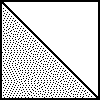
\includegraphics{arrays_matrix-bl.png}

Элементы на диагональных линиях считаются принадлежащими этой области.

\section{Оборудование студента}
\mypc

\section{Программное обеспечение}
VIM + утилита clisp из репозиториев дистрибутива.

\section{Идея, метод, алгоритм}
\section{Сценарий выполнения работы}
\section{Распечатка программы и её результаты}

\subsection{Исходный код}
\listsource{..}{lab3.lisp}
\listsource{..}{main.lisp}

\subsection{Результаты работы}
\lstinline{clisp -i lab3.lisp main.lisp > log.lisp}
\listsource{..}{log.lisp}

\section{Дневник отладки}
\noindent
\begin{tabularx}{\linewidth}{|c|X|X|X|}
\hline
Дата & Событие & Действие по исправлению & Примечание \\
\hline
08/08/2020 & На последнем тесте выдало число 9999 & В функции {\tt matrix-elem} поменял местами индексы элемента & Тесты круто \\
\hline
\end{tabularx}

\section{Замечания автора по существу работы}

\section{Выводы}

\end{document}
